\chapter{Swalbe.jl: A lattice Boltzmann solver for thin film hydrodynamics}
\label{chapter:fourth_paper}
\epigraph{\textit{Okay die Eisbären gehen unter denn der Wasserspiegel steigt, ist mir egal in meinem Baccardi ist noch Eis}}{Neodisco}

\textit{\small{This chapter has been submitted as a regular contribution to the Journal of open source software. The review process is performed under the issue number \href{https://github.com/openjournals/joss-reviews/issues/3728}{3728}}}

\section{Summary}

Small amounts of liquid deposited on a substrate are an everyday phenomenon.
From a theoretical point of view this represents a modelling challenge, due to the multiple scales involved: from the molecular interactions among the three phases (solid substrate, liquid film and surrounding gas) to the hydrodynamic flows.
An efficient way to deal with this problem is via the thin-film equation:
\begin{equation}\label{eq:thin_film_Joss}
    \partial_t h = \nabla\cdot(M(h)\nabla p),
\end{equation}
where $h$ is the film thickness, $M(h)$ is a thickness dependent mobility and $p$ is the pressure inside the film.
Solving the thin film equation directly is however a difficult task as it is a fourth order degenerate PDE~\cite{becker2003complex}.
\textit{Swalbe.jl} approaches the problem from a different angle.
Instead of directly solving the thin film equation we use a novel method based on a class lattice Boltzmann models~\cite{krueger2017}, originally developed to simulate shallow water flows~\cite{Salmon:1999:0022-2402:503}.
This allows us to benefit from the simplicity of the lattice Boltzmann algorithm which makes it straightforward to parallelize the code and run it on accelerator devices.
Choosing appropriate forces it is possible to simulate complex problems.
Among them is the dewetting of a patterned substrates as shown in Fig.~\ref{fig:logo}.
It is as well possible to simulate low contact angle droplets out of equilibrium to probe relaxation experiments, e.g. the Cox-Voinov or Tanner's law~\cite{RevModPhys.81.739}.
Due to a disjoining pressure model for the three phase contact line droplets can not only relax towards their equilibrium they can slide as well~\cite{PhysRevE.100.033313}.
All of this can be coupled with thermal fluctuations to study the stochastic thin film equation~\cite{shah_van_steijn_kleijn_kreutzer_2019}.

\begin{figure}
    \centering
    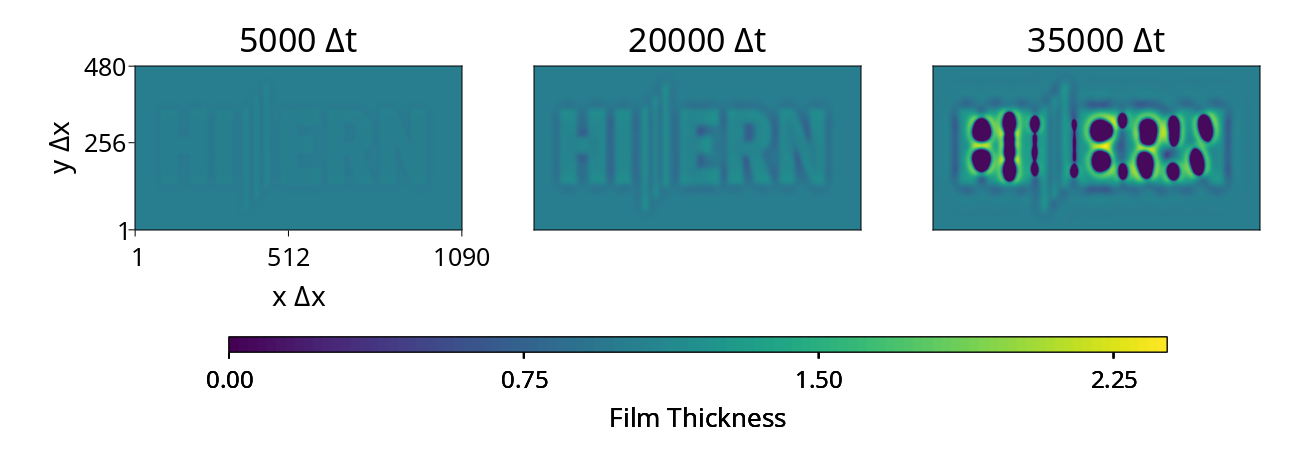
\includegraphics[width = 0.9\textwidth]{graphics/Hiern_logo.png}
    \caption{Dewetting simulation on a patterned substrate, letters have a higher wettability than the rest of the substrate.}
    \label{fig:logo}
\end{figure}

\section{Statement of need}

\textit{Swalbe} is written in Julia~\cite{doi:10.1137/141000671} and developed for a \textit{script your experiment} workflow.
For that reason an experiment is composed of three steps.
First, the initial problem is defined by setting the system size and other input parameters, stored in a custom type.
Followed by the lattice Boltzmann time loop where different force terms allow for different dynamics.
To note here however is that some forces are mandatory for every experiment.
This is on the one hand the friction with the substrate, the slip that helps regularizing the contact line and on the other hand the capillary- or filmpressure that accounts for the correct wetting behavior.  
After the time loop has ended an IO step can be included to store the data in files or to generate a plot.
The package is written in pure Julia, therefore it can be easily coupled with other packages from the Julia ecosystem such as Plots.jl~\cite{tom_breloff_2021} to visualize data and JLD2.jl~\cite{JLD2.jl} to store data in HDF5 format.
Of course one future development goal is to interact with \textit{SciML} environment to pair modelling with ML.  
\textit{Swalbe.jl} is designed to approach two problems, first being the modelling itself and second the applicability to large system sizes.
Ideas can be implemented quickly and tested with a two dimensional system, which is discretized in a single horizontal direction and offers a second computed dimension for the thickness.
The hardware requirements to run these two dimensional simulations are comparably low and depending on the number of lattice Boltzmann iterations ranging from seconds to at most an hour on a single Core of a modern CPU.
After testing it is possible to scale up and simulate the same or other problems in three dimensions with a slightly more complex discretization.
Keeping the simulation time low is archived by using a Nvidia GPU.
Most functions are written in a generic style and can be executed both on a CPU or GPU.
For the GPU usage the high-level API of CUDA.jl~\cite{besard2018juliagpu, besard2019prototyping} is used, mostly CuArrays.

An older version of the numerical model (written in C++) has been tested and used for thin film simulations in previous publications~\cite{PhysRevE.100.033313, PhysRevE.104.034801}.
While there is a small performance decrease when moving from C++ with OpenACC to Julia, the benefits of usability, straightforward documentation and automated testing outweighs this issue.
There are many thin film problems the authors will investigate in the future with \textit{Swalbe.jl}.
Among those are switchable substrate and their influence on a dewetting thin film, or the influence of thermal fluctuations on the coalescence of droplets.

\section{State of the field}

In the context of computational fluid dynamics low Reynolds number flows and especially thin film flows are a comparably small subsection.
Therefore numerical tools that deal exclusively with the thin film problem are sparse.
Two packages for simulations of thin film hydrodynamics are \textbf{ThinViscoelasticFilms} and \textbf{stochastic\_thin\_films}~\cite{ThinViscoelasticFilms, stochastic_thin_films}.
The core components are written in \textit{Fortran} and at least the later package can be used according to BSD-2 license.
Documentation however is only available through code comments and a short readme, leaving the user little guidance.

That said, the thin film equation is a fourth-order parabolic equation and can of course be solved with appropriate numerical schemes.
Some of these schemes can be found in the refs.~\cite{PhysRevFluids.1.073901, PhysRevE.63.011208, becker2003complex, Peschka9275}.
Upon contacting the authors it should be possible to have access to a working version of the described approach.

Wilczek et al. used \href{https://www.dune-project.org/}{\textbf{DUNE}} to study the dynamics of an ensemble of sliding drops in ref.~\cite{PhysRevLett.119.204501}.
DUNE is a software suite written in \textit{C++} that solves partial differential equations with a grid based approach~\cite{sander2020dune}.
Therefore DUNE is not limited to the problem of thin film flows, interested readers may visit the project's home page.

Another open source package with similar functionality that is used to solve thin film problems is \href{http://oomph-lib.maths.man.ac.uk/doc/html/index.html}{\textbf{oomph-lib}}.
oomph-lib uses both \textit{Fortran} as well \textit{C} components to solve differential equations.
The library's emphasis however are fluid dynamic problems as can be seen from refs.~\cite{heil2015flow, pihler2015displacement, pihler2013modelling}.
Of course, similar to DUNE, its capabilities are not limited to thin film problems.

Given the nature of the thin film problem one can, as well, use classical Navier-Stokes solvers with appropriate initial and boundary conditions.
What comes to mind here is for example \href{https://www.openfoam.com/}{\textbf{OpenFOAM}} a widely used open source CFD software with an active community.
Another example utilizing a Navier-Stokes solver would be the \href{http://basilisk.fr}{\textbf{basilisk}} software library, which is written in \textit{C} and is the successor of \href{http://gfs.sourceforge.net/wiki/index.php/Main_Page}{\textbf{GERRIS}}.

Lattice Boltzmann solvers offer another category to approximate the Navier-Stokes equation.
Starting point of this method is not the Navier-Stokes equation but the Boltzmann equation.
Using the Chapman-Enskog expansion~\cite{Chapman, Enskog}, it can be shown that the resulting system of equations recovers to the Navier-Stokes equation.
The method is straightforward to implement and several small to large projects can be found with OSI-approved license. 
To name just a few examples: \href{https://walberla.net/doxygen/index.html}{\textbf{waLBerla}}, \href{https://www.openlb.net/}{\textbf{openLB}} or some smaller project \href{https://gitlab.com/unigehpfs/stlbm}{\textbf{STLBM}}. 

Proprietary software, e.g. \href{https://www.comsol.com/}{\textbf{COMSOL}} can as well be used to simulate thin film dynamics.
Wedershoven et al. used COMSOL to study the rupture of a thin film due to laser irradiation~\cite{doi:10.1063/1.4863318}.
Berendsen et al. from the same group simulated the dynamics an impinging air jet has on a thin film using COMSOL~\cite{doi:10.1021/la301353f}.

With the exclusion of \textbf{ThinViscoelasticFilms} every above mentioned project has a much wider purpose than \textit{just} solving the thin film equation.
However due to the generality of most libraries it can become quite complex to set up a simulation for a thin film problem.
Especially concerning the Navier-Stokes solvers one uses a \textit{sledge hammer to crack a nut}.

\section{Use Case}

An interesting problem in the domain of thin liquid films is the coalescence of sessile droplets, see references~\cite{eggers1999coalescence, PhysRevLett.111.144502, PhysRevLett.109.184502, PhysRevLett.95.164503}.
The underlying idea is that two droplets placed on a hydrophilic substrate in close contact to each other will coalesce into a single droplet to minimize their surface area and therefore energy.
The dynamics of this process can be explained using a self-similarity solution of the thin film equation.
In fact, that the bridge height, the point that connects the two droplets, has to grow with a power law.
We now show how to perform that simulation with the help of the \textit{Swalbe.jl} package.
The goal will be to observe a growth of the bridge height as 
\begin{equation}\label{eq:powerlaw}
    h_0(t) = k t^{\alpha},
\end{equation}
where the exponent $\alpha$ should be $2/3$~\cite{doi:10.1063/1.5119014, doi:10.1063/1.4824108}.
This experiment has been performed using the \textit{Pluto notebook} \href{https://jugit.fz-juelich.de/compflu/swalbe.jl/-/blob/JOSS/scripts/Drop_coal.jl}{Drop\_coal.jl}.

Just to outline the most important steps towards the simulation:
\begin{enumerate}
\item Define the initial conditions of the simulation
\item Define a function that performs the experiment
\item Run the experiment with varying parameters:
\begin{minted}{julia}
for gamma in enumerate(gammas)
  # System parameter, delta=50 can still considered small to  
  # medium slippage (delta approx max(height))
  sys = Swalbe.SysConst_1D(L=1024, 
                           Tmax=2000000, 
                           delta=50.0, 
                           gamma=gamma[2]
                          )
  # The experiment
  data_merge[:,:,gamma[1]] = run_drop_coal(sys, 
                                           r1=sphere_rad, 
                                           r2=sphere_rad
                                          )
end
\end{minted}
\item Display the results, see Fig.~\ref{fig:coalesence} 
\end{enumerate}

\begin{figure}
    \centering
    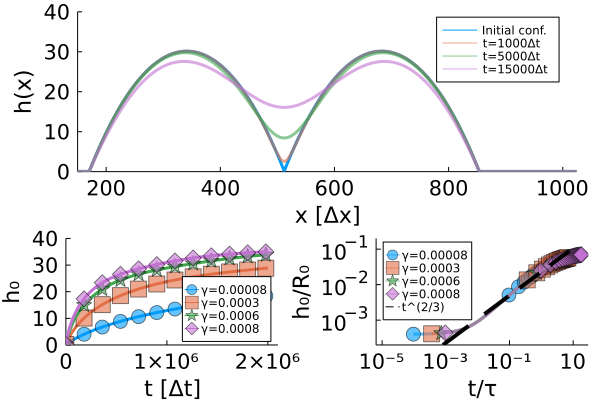
\includegraphics[width = 0.75\textwidth]{graphics/drop_coal.png}
    \caption{Coalescence of sessile droplets on a partially wetting substrate. The upper panel shows the time evolution for a single experiment (lowest surface tension). In the lower left panel we plot the evolution of the bridge height for the four different surface tensions. To the right we normalize the data with characteristic quantities and show that the bridge height grows as $\propto t^{2/3}$.}
    \label{fig:coalesence}
\end{figure}

\section{Acknowledgements}

The authors acknowledge financial support by the Deutsche Forschungsgemeinschaft (DFG) within the priority program SPP2171 ``Dynamic Wetting of Flexible, Adaptive, and Switchable Substrates'', within project HA-4382/11.